\documentclass[]{elsarticle} %review=doublespace preprint=single 5p=2 column
%%% Begin My package additions %%%%%%%%%%%%%%%%%%%
\usepackage[hyphens]{url}

  \journal{Lancet: Global Health} % Sets Journal name


\usepackage{lineno} % add
  \linenumbers % turns line numbering on
\providecommand{\tightlist}{%
  \setlength{\itemsep}{0pt}\setlength{\parskip}{0pt}}

\usepackage{graphicx}
\usepackage{booktabs} % book-quality tables
%%%%%%%%%%%%%%%% end my additions to header

\usepackage[T1]{fontenc}
\usepackage{lmodern}
\usepackage{amssymb,amsmath}
\usepackage{ifxetex,ifluatex}
\usepackage{fixltx2e} % provides \textsubscript
% use upquote if available, for straight quotes in verbatim environments
\IfFileExists{upquote.sty}{\usepackage{upquote}}{}
\ifnum 0\ifxetex 1\fi\ifluatex 1\fi=0 % if pdftex
  \usepackage[utf8]{inputenc}
\else % if luatex or xelatex
  \usepackage{fontspec}
  \ifxetex
    \usepackage{xltxtra,xunicode}
  \fi
  \defaultfontfeatures{Mapping=tex-text,Scale=MatchLowercase}
  \newcommand{\euro}{€}
\fi
% use microtype if available
\IfFileExists{microtype.sty}{\usepackage{microtype}}{}
\bibliographystyle{elsarticle-harv}
\usepackage{longtable}
\ifxetex
  \usepackage[setpagesize=false, % page size defined by xetex
              unicode=false, % unicode breaks when used with xetex
              xetex]{hyperref}
\else
  \usepackage[unicode=true]{hyperref}
\fi
\hypersetup{breaklinks=true,
            bookmarks=true,
            pdfauthor={},
            pdftitle={S1 Data Collection Protocols for Combining Rapid Antigen Testing and Syndromic Data Improves Sensitivity and Specificity in Real-World COVID-19 Detection},
            colorlinks=false,
            urlcolor=blue,
            linkcolor=magenta,
            pdfborder={0 0 0}}
\urlstyle{same}  % don't use monospace font for urls

\setcounter{secnumdepth}{5}
% Pandoc toggle for numbering sections (defaults to be off)

% Pandoc citation processing

% Pandoc header
\renewenvironment{abstract}{}{}
\usepackage[colorinlistoftodos]{todonotes}
\usepackage{pdfpages}



\begin{document}
\begin{frontmatter}

  \title{\textbf{S1 Data Collection Protocols} for \emph{Combining Rapid Antigen Testing and Syndromic Data Improves Sensitivity and Specificity in Real-World COVID-19 Detection}}
    \author[IBAHCM,UoGLMICS]{Fergus J Chadwick}
   \ead{f.chadwick.1@research.gla.ac.uk} 
    \author[IBAHCM,UoGLMICS]{Yacob Haddou}
   \ead{yacob.haddou@glasgow.ac.uk} 
    \author[IBAHCM]{Tasnuva Chowdhury}
   \ead{tasnuvachowdhury2004@gmail.com} 
    \author[MRCB]{David Pascall}
   \ead{david.pascall@mrc-bsu.cam.ac.uk} 
    \author[a2i]{Shayan Chowdhury}
   \ead{shayan.chowdhury@a2i.gov.bd} 
    \author[IBAHCM,UoGLMICS]{Jessica Clark}
   \ead{Jessica.Clark@glasgow.ac.uk} 
    \author[UNFAO]{Joanna Andrecka}
   \ead{aandrecka@gmail.com} 
    \author[MathsandStatGla,UoGLMICS]{Mikolaj Kundergorski}
   \ead{mikolaj.kundegorski@gmail.com} 
    \author[MathsandStatGla,UoGLMICS]{Craig Wilkie}
   \ead{craig.wilkie@glasgow.ac.uk} 
    \author[UNFAO]{Eric Brum}
   \ead{eric.brum@fao.org} 
    \author[IEDCR]{Tahmina Shirin}
   \ead{tahmina.shirin14@gmail.com} 
    \author[IEDCR]{A S M Alamgir}
   \ead{aalamgir@gmail.com} 
    \author[IEDCR]{Mahbubur Rahman}
   \ead{dr\_mahbub@yahoo.com} 
    \author[IEDCR]{Ahmed Nawsher Alam}
   \ead{anawsher@yahoo.com} 
    \author[IEDCR]{Farzana Khan}
   \ead{farzanakhan\_25@yahoo.com} 
    \author[MathsandStatGla,UoGLMICS]{Janine Illian}
   \ead{janine.illian@glasgow.ac.uk} 
    \author[MathsandStatGla,UoGLMICS]{Ben Swallow}
   \ead{ben.swallow@glasgow.ac.uk} 
    \author[IBAHCM,UoGLMICS]{Davina L Hill}
   \ead{davina.hill@glasgow.ac.uk} 
    \author[MathsandStatGla]{Dirk Husmeier}
   \ead{dirk.husmeier@glasgow.ac.uk} 
    \author[IBAHCM,UoGLMICS]{Jason Matthiopoulos}
   \ead{jason.matthiopoulos@glasgow.ac.uk} 
    \author[IBAHCM,UoGLMICS]{Katie Hampson}
   \ead{katie.hampson@glasgow.ac.uk} 
    \author[Columbia]{Ayesha Sania}
   \ead{ays328@mail.harvard.edu} 
      \address[IBAHCM]{Institute of Biodiversity, Animal Health and Comparative Medicine, University of Glasgow}
    \address[UoGLMICS]{COVID-19 in LMICs Research Group, University of Glasgow}
    \address[MRCB]{MRC Biostatistics Unit, University of Cambridge}
    \address[MathsandStatGla]{School of Mathematics and Statistics, University of Glasgow}
    \address[a2i]{a2i, United Nations Development Program, ICT Ministry, Bangladesh}
    \address[UNFAO]{UN FAO in support of the UN Interagency Support Team, Bangladesh}
    \address[IEDCR]{Institute of Epidemiology, Disease Control and Research, Ministry of Health, Bangladesh}
    \address[Columbia]{Division of Developmental Neuroscience, Department of Psychiatry, Columbia University}
      \cortext[1]{Corresponding Author}
  
  \begin{abstract}
  
  \end{abstract}
  
 \end{frontmatter}

This document compiles the Community Support Teams' Standard Operating Procedures for the identification of potential COVID-19 patients, screenshots of the data-collection application, and the protocol for the taking of nasal swabs for rapid antigen and PCR testing.

\hypertarget{guidelines-for-identification-of-potential-virus-fighters-pvf.}{%
\section{Guidelines for Identification of Potential Virus Fighters (PVF).}\label{guidelines-for-identification-of-potential-virus-fighters-pvf.}}

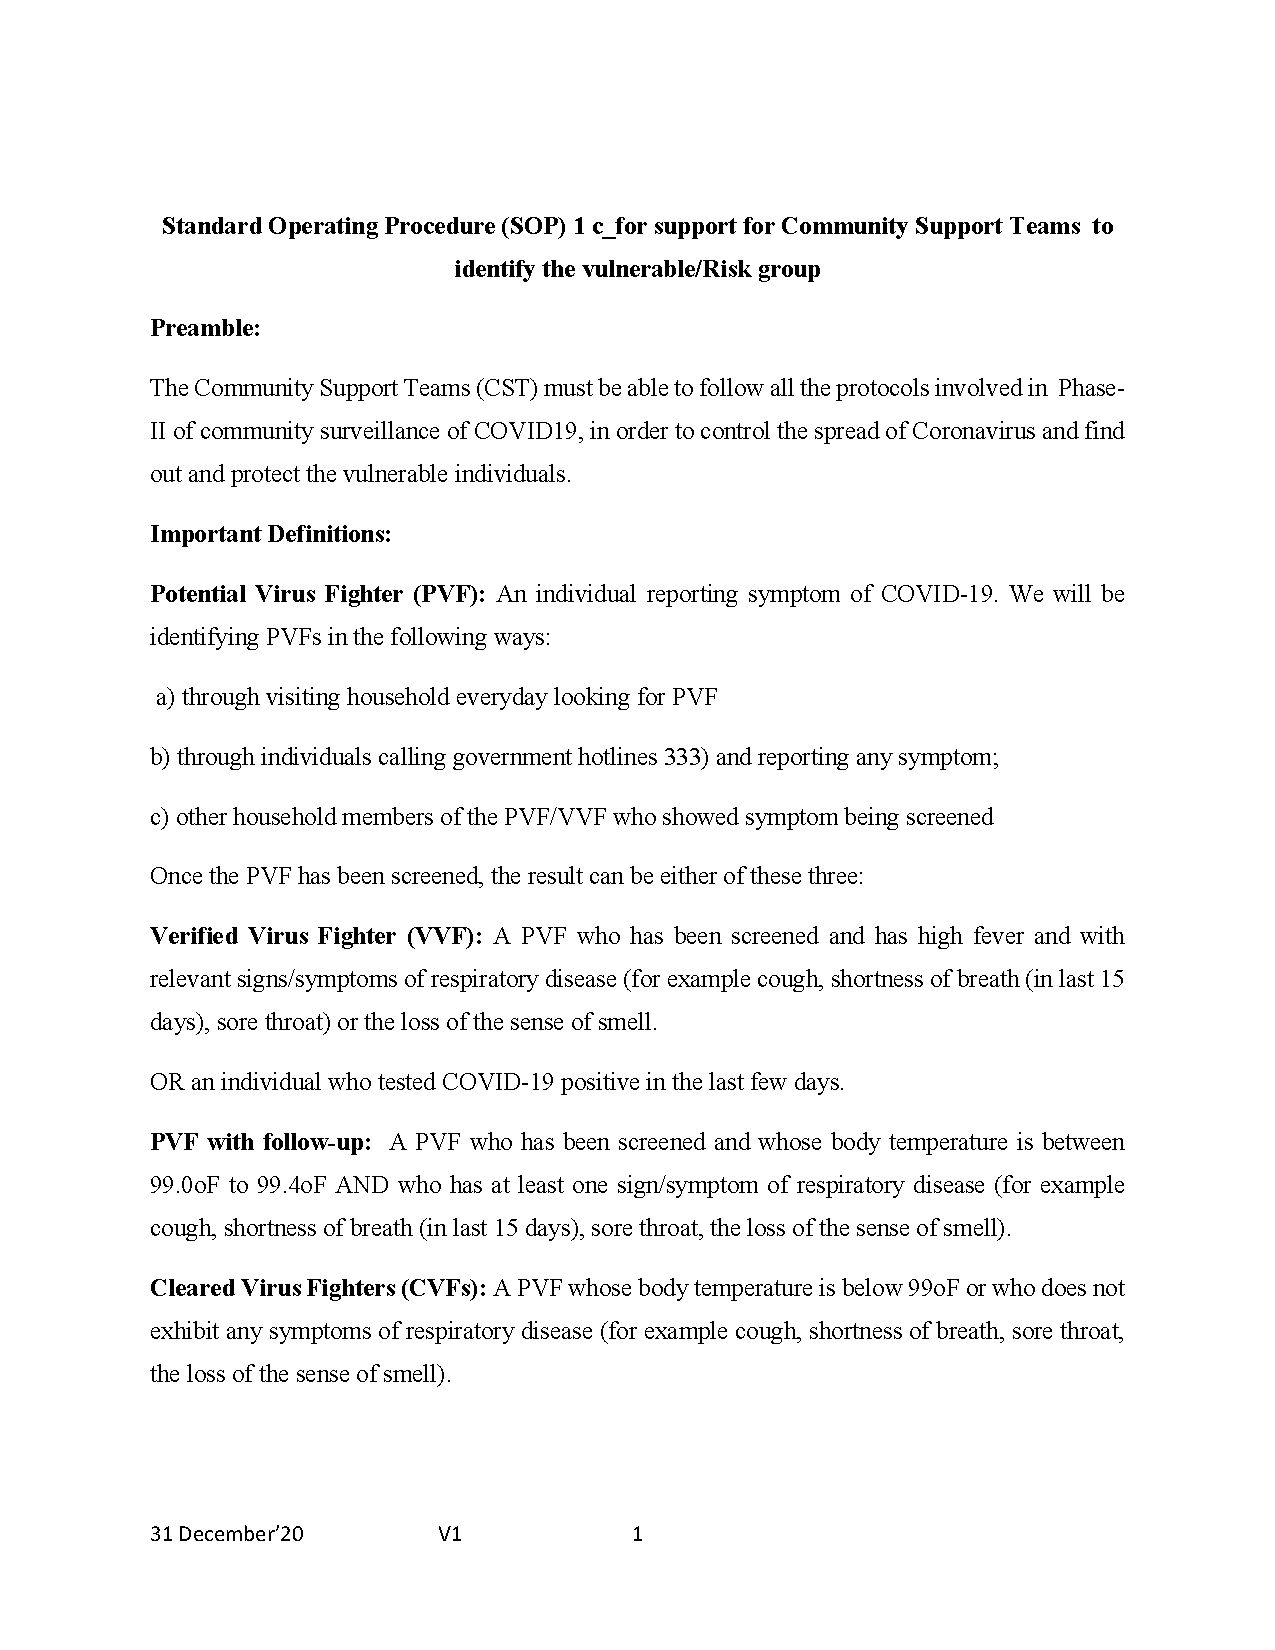
\includepdf[pages={-}]{Supp1Figs/SOP1.pdf}
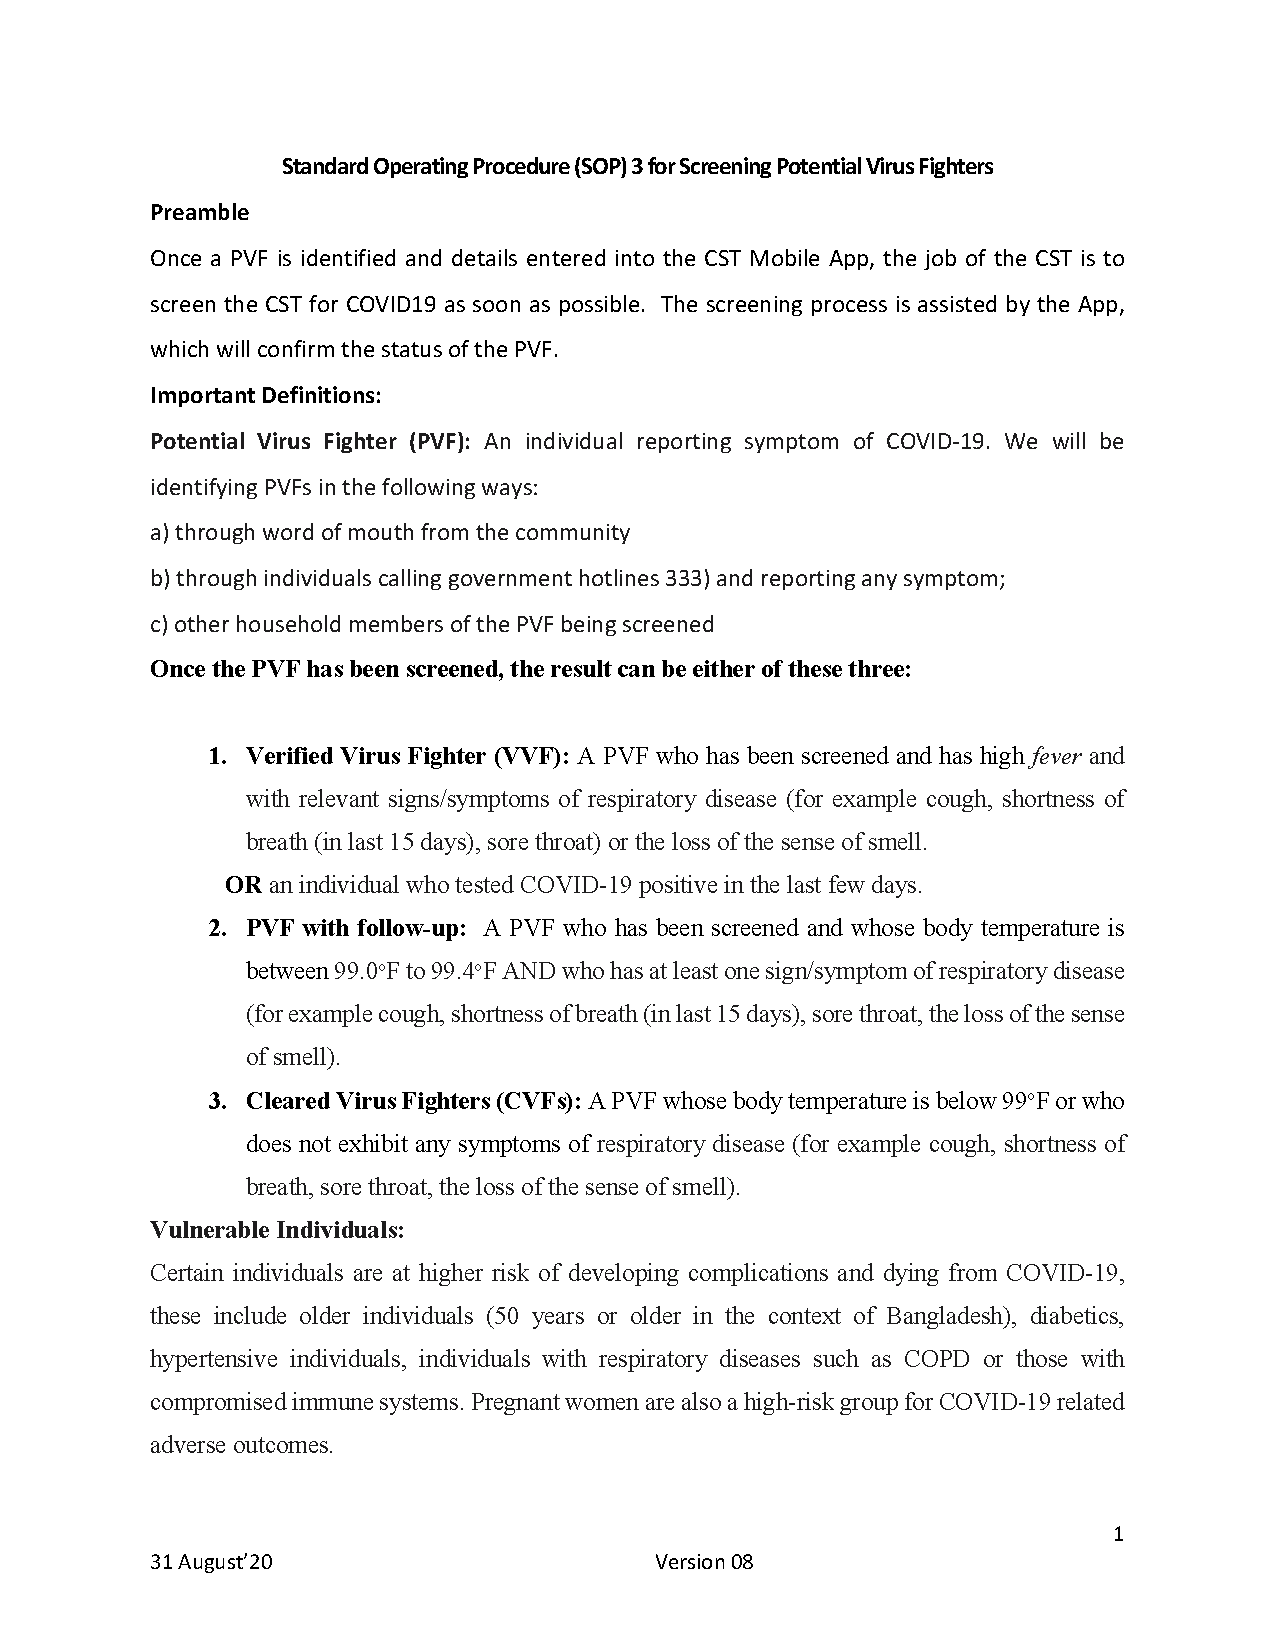
\includepdf[pages={-}]{Supp1Figs/SOP3.pdf}
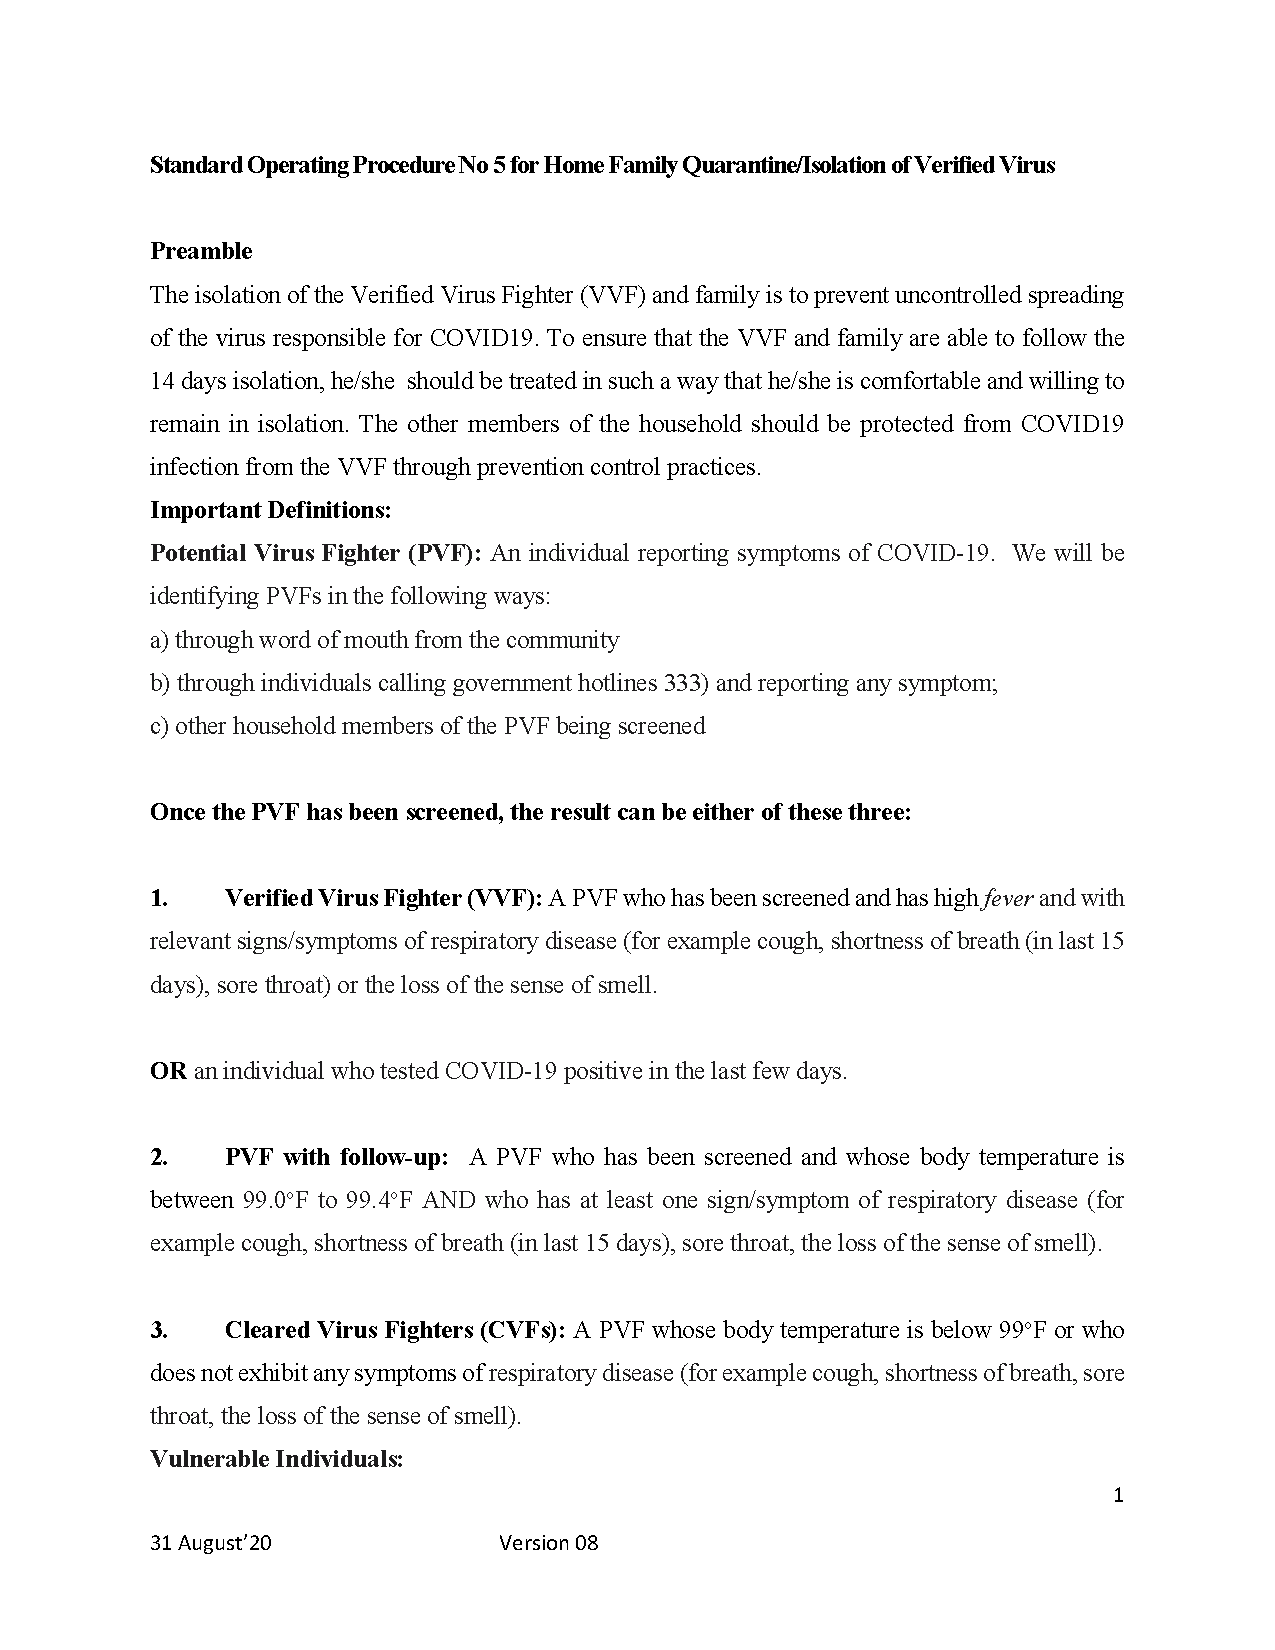
\includepdf[pages={-}]{Supp1Figs/SOP5.pdf}

\hypertarget{data-collection-application}{%
\section{Data Collection Application}\label{data-collection-application}}

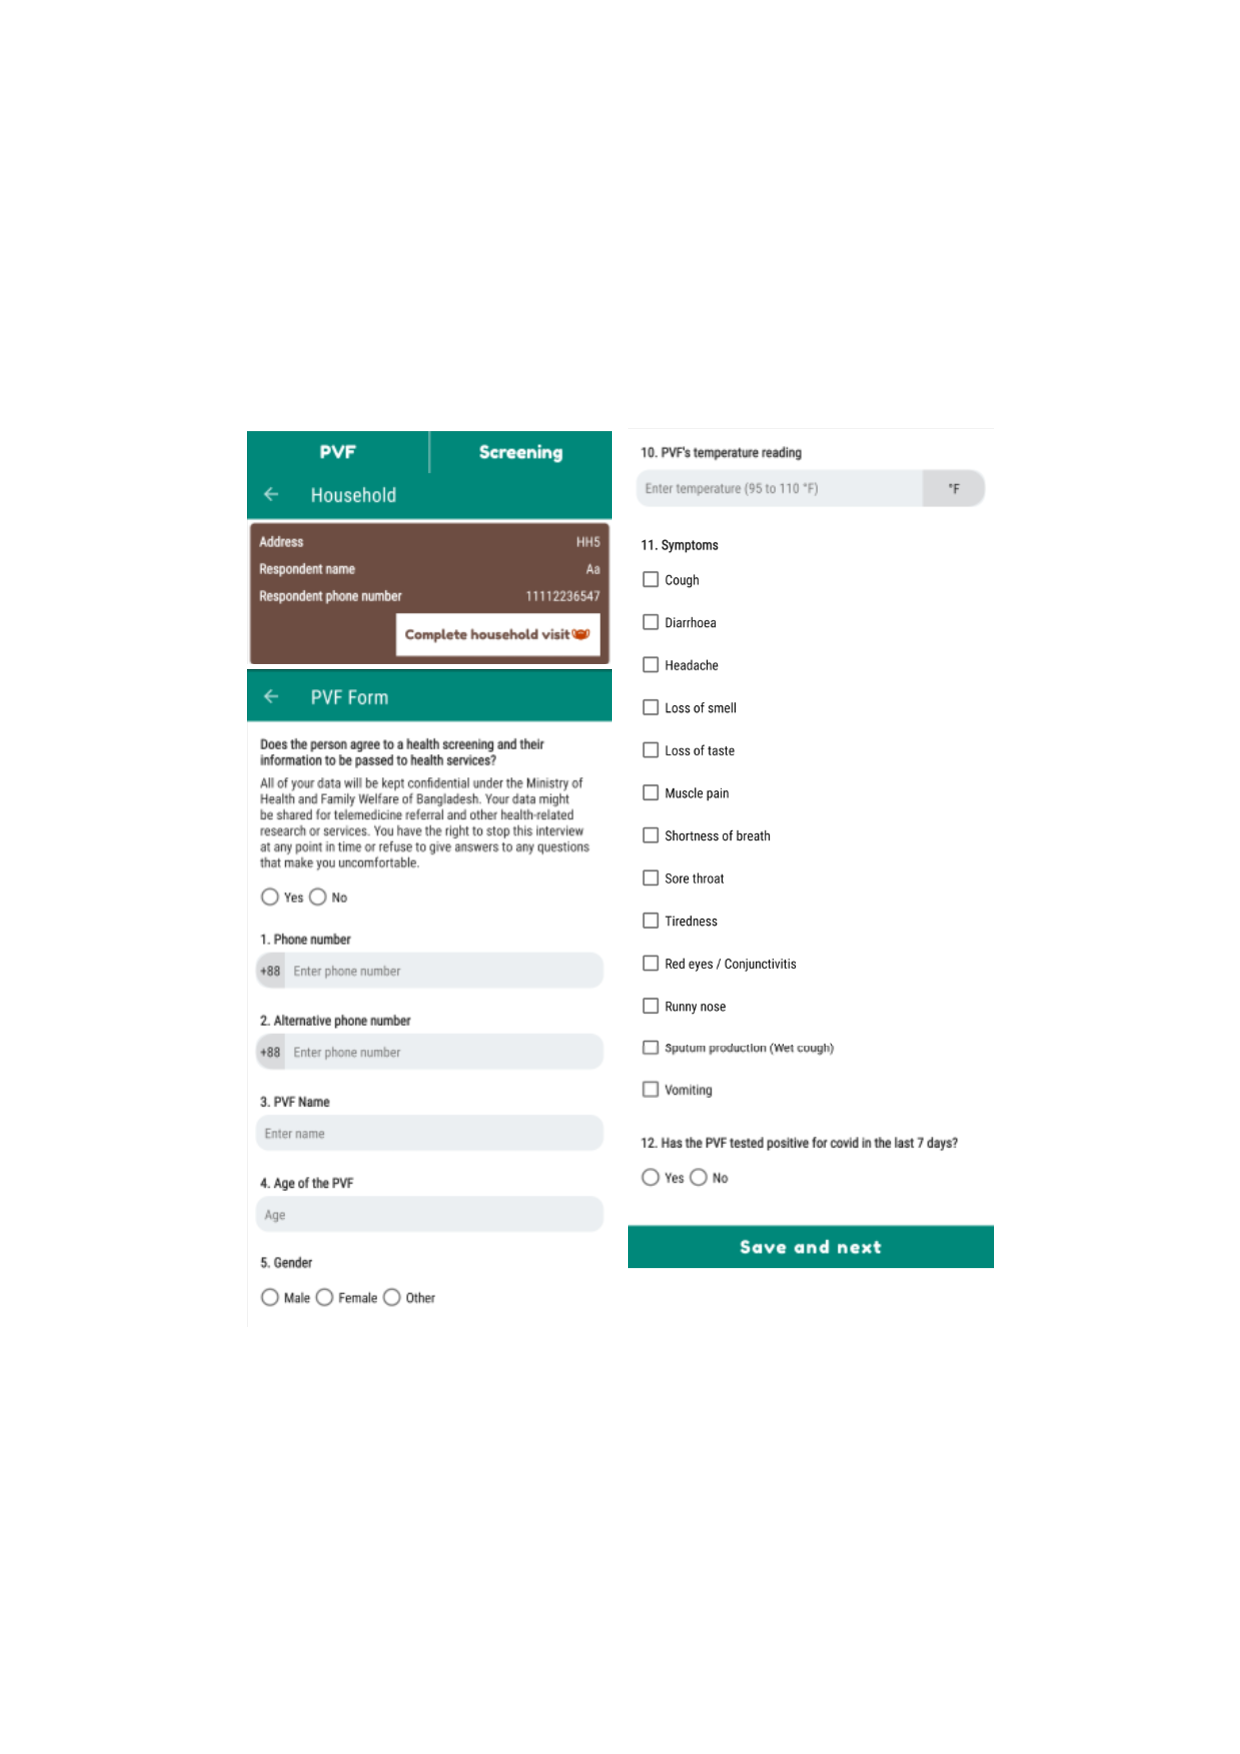
\includepdf[pages={-}]{Supp1Figs/app_screenshots.pdf}

\hypertarget{sample-and-swab-collection-protocol}{%
\section{Sample and Swab Collection Protocol}\label{sample-and-swab-collection-protocol}}

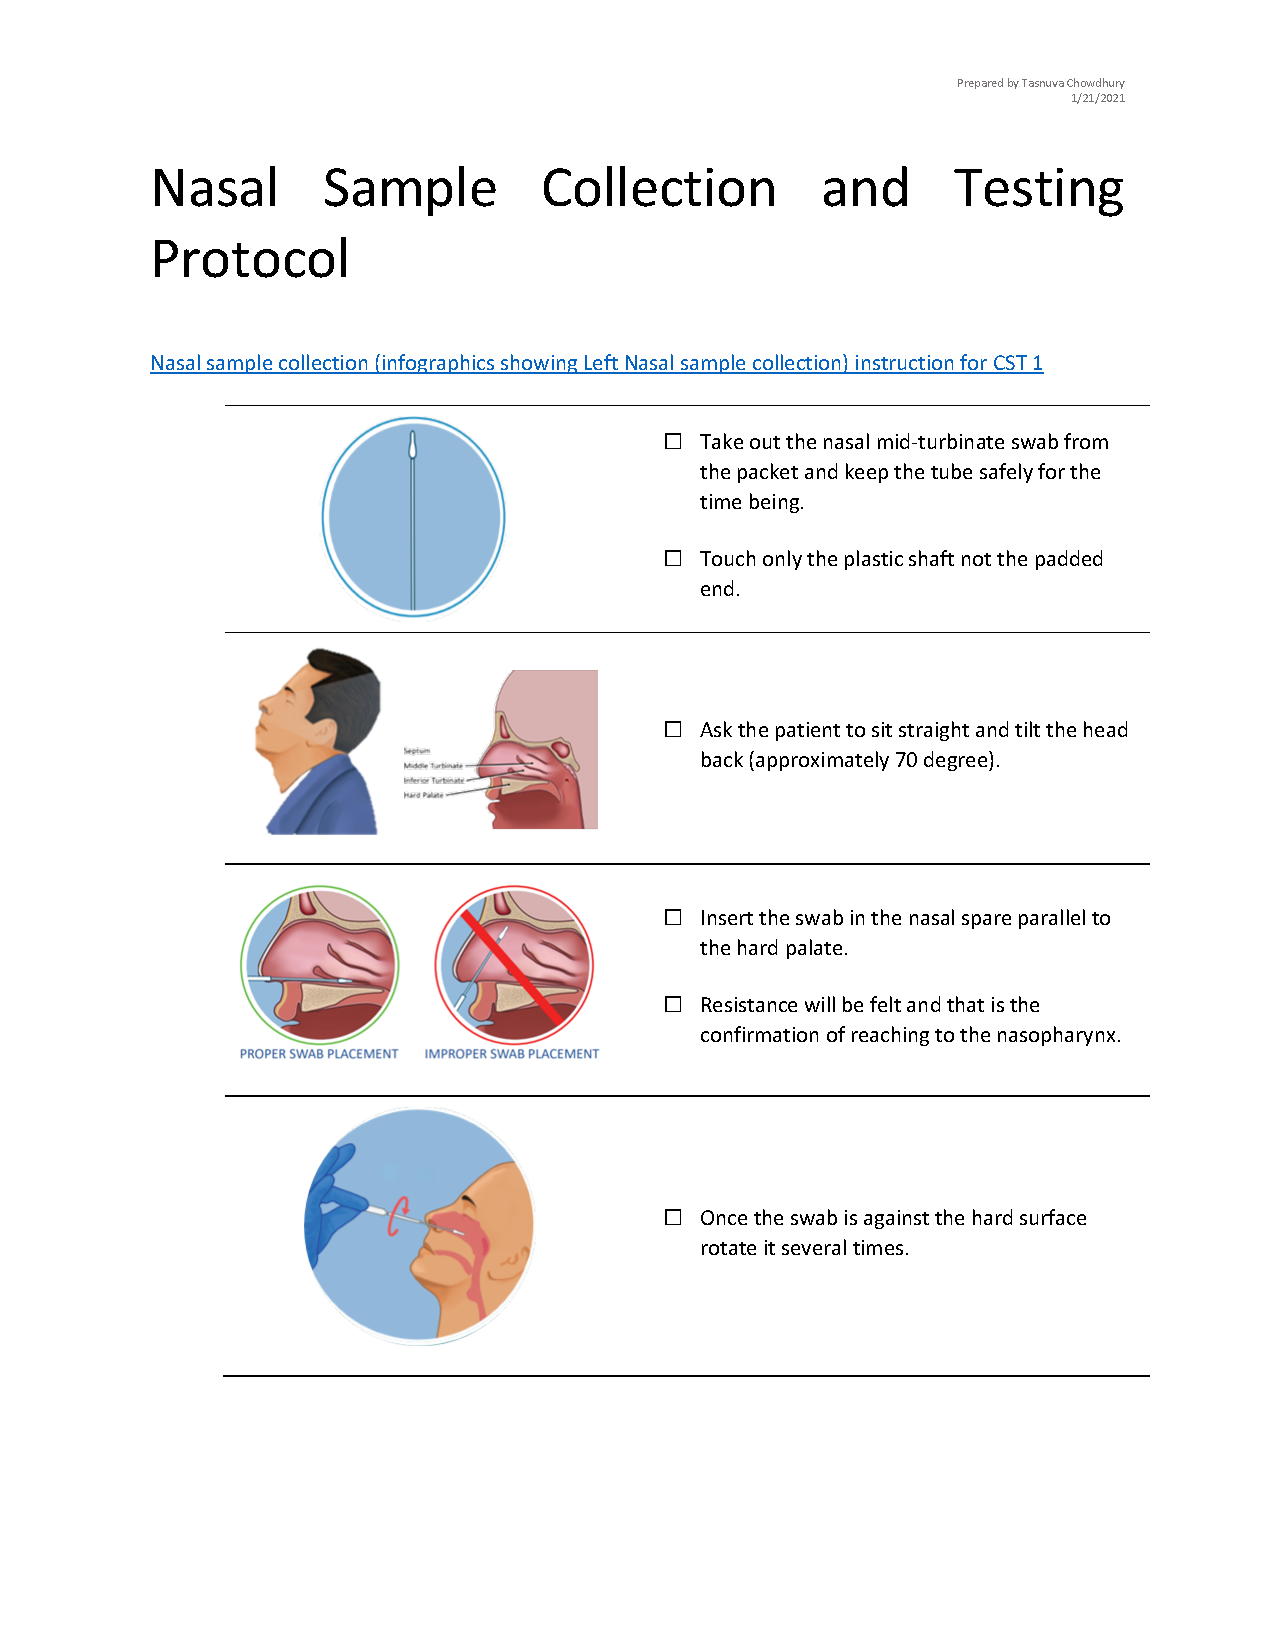
\includepdf[pages={-}]{Supp1Figs/SampleProtocol.pdf}


\end{document}
